\documentclass[a4paper]{article}

%% Language and font encodings
\usepackage[english]{babel}
\usepackage[utf8x]{inputenc}
\usepackage[T1]{fontenc}

%% Sets page size and margins
\usepackage[a4paper,top=3cm,bottom=2cm,left=3cm,right=3cm,marginparwidth=1.75cm]{geometry}

%% Useful packages
\usepackage{amsmath}
\usepackage{graphicx}
\usepackage{subfig}
\usepackage[colorinlistoftodos]{todonotes}
\usepackage[colorlinks=true, allcolors=blue]{hyperref}

\title{Reporte de Activdad 5}
\author{Valenzuela Terán Jonás}

\begin{document}
\maketitle
%---------------------------------------------------------------------------

\section{Introducción a la Actividad}

Uno de los pasos más importantes en el análisis de datos es la limpieza de ellos, y crear un formato que sea legible por las herramientas que se utilizarán, en este caso, pandas. Para la limpieza se hace uso de emacs, ya que ofrece comandos que permiten automatizar ciertos procesos de edición de texto plano, lo cuál permite cambiar el formato de un archivo extenso con pocas instrucciones, y poco tiempo. 

\begin{center}

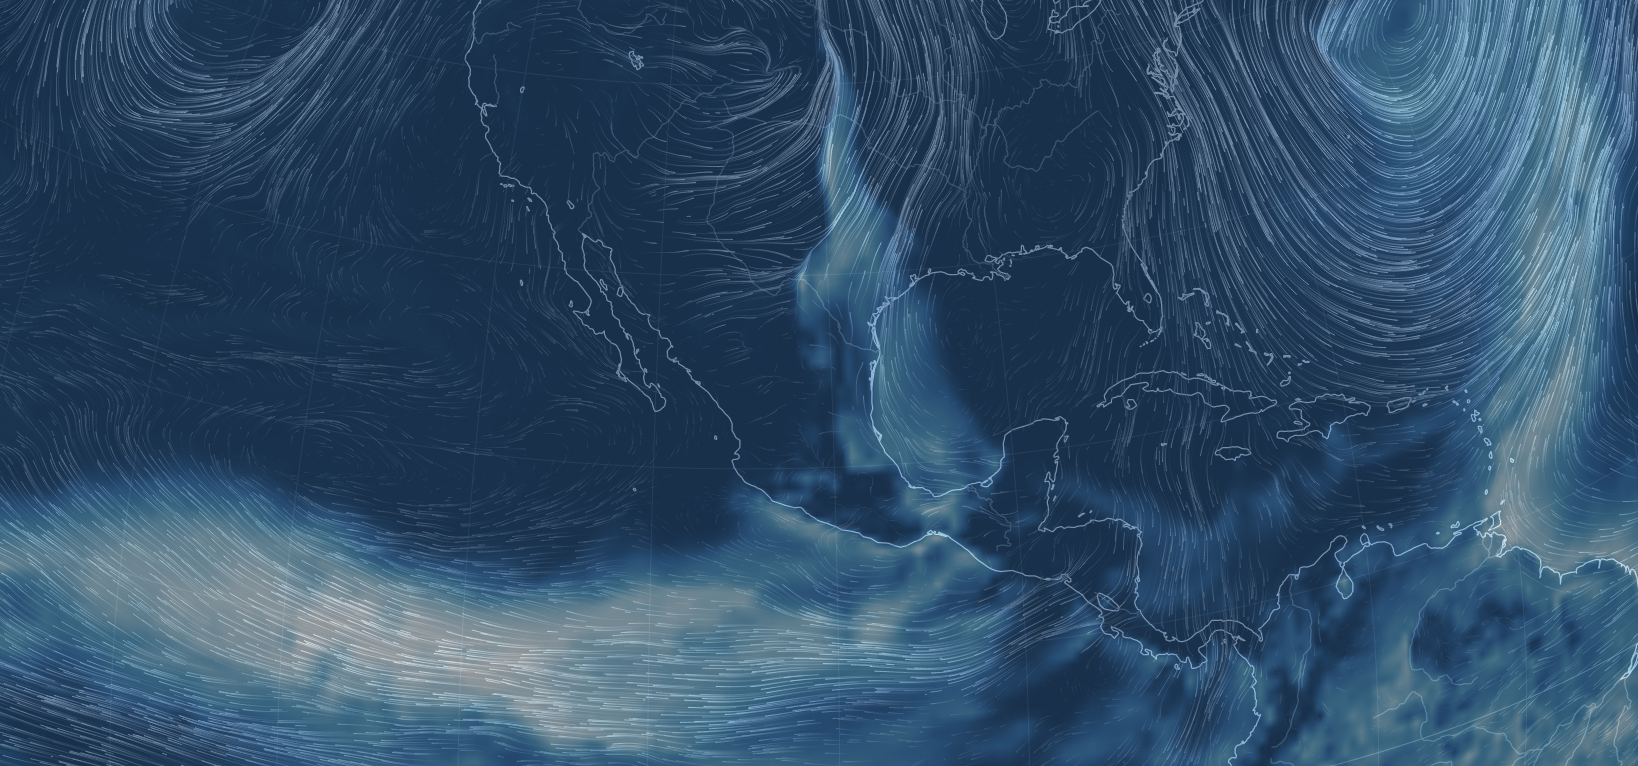
\includegraphics[height=6cm]{rep5.PNG}

Fuente: \textit{https://earth.nullschool.net/\#current/wind/surface/level/orthographic=-93.80,17.09,671}

\end{center}

Los datos tomados describen sondeos de la Atmósfera de la Universidad de Wyoming, se enfocará específicamente en CAPE y PW, con el interés de encontrar una relación entre ambos parámetros.

\section{Convective Available Potential Energy y Precipitable Water}

	\subsection{CAPE (Convective Available Potential Energy)}

Es la capacidad de energía que una muy pequeña cantidad de aire poseería si fuera elevado por la atmósfera verticalmente. Es útil para indicar inestabilidad atmosférica, que pronostica climas peligrosos. 

Es medido en la troposfera, su unidad es Joules por kilogramo (J/Kg), cualquier valor mayor a 0 J/Kg indica inestabilidad y mayor posibilidad de tormentas (Debe existir vapor de agua).

	\subsection{PW (Precipitable Water)}

Comúnmente abreviado como "TPW" = Total Precipitable Water,   es la profundidad de agua en una columna de atmósfera, si toda el agua en la columna fuera precipitada en lluvia. Es medida en milímetros. 


\section{Procesamiento y limpieza de datos}

Primero se cargaron los datos de la Universidad de Wyoming, de sondeos atmosféricos de Empalme, Sonora, a las 00:00 y 12:00 horas, usando un script construido en actividades anteriores, una vez obtenidos, en la terminal, se recolecta toda la información en un solo archivo csv, utilizando el comando cat.

Se sigue con la limpieza de datos en emacs, borrando newlines, información que no corresponde con la fecha, CAPE y PW que son de interés, se agregan comas para separar estas categorias y newlines para cada medición, creando un formato legible para pandas usando python, esto es posible gracias a la automatización de acciones que ofrece emacs sobre un patrón indicado, el procedimiento consistió en:

\begin{itemize}
\item Seleccionar patrón (Ctrl + SPACE)
\item Cortar y pegar información para guardar en memoria (Ctrl + w) y (Ctrl + y)
\item Ir al inicio del archivo (Esc + <)
\item Entrar al modo del comando (Esc + SHIFT + \%)
\item Insertar el patrón (Esc + y) (Enter)
\item Insertar remplazo del patrón (Insertar reemplazo) (Enter)
\item Aplicar (!)
\end{itemize}

\section{Análisis de datos}

Una vez preparados los archivos, uno para mediciones en 00:00 y otro para 12:00 horas, se leyeron y asignaron a un dataframe en python, usando el entorno de programación jupyter notebook e importando librerias como pandas y numpy para herramientas estadísticas y numéricas, y datetime para detectar correctamente el formato de la fecha.

Esto hace posible la representación gráfica de los datos usando las herramientas disponibles de las bibliotecas, y ver claramente si existe una relación entre CAPE y PW. Realizamos 3 tipos de representación: boxplot, PW contra CAPE, PW contra CAPE con colores indicando mes.


\section{Resultados}

A continuación se muestran las gráficas obtenidas por el programa, la primera imagen corresponde a las mediciones de las 00:00 horas, y la segunda a las 12:00 horas:

\begin{center}
	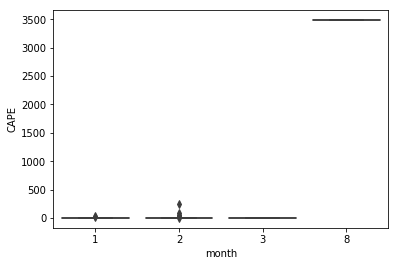
\includegraphics[height=5cm]{Z001.png}
    
    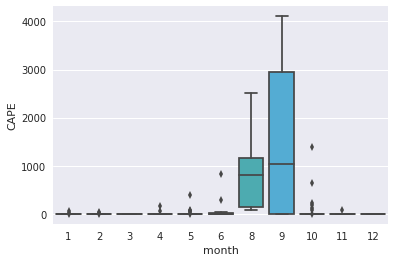
\includegraphics[height=5cm]{Z121.png}
    
    \textit{Boxplots de CAPE en cada mes}
\end{center}

Se observa la ausencia de mediciones a las 00:00 horas. A las 12:00 horas, CAPE se mantiene reducido durante todo el año, a excepción de agosto y septiembre, donde existe una fuerte elevación.

\begin{center}
	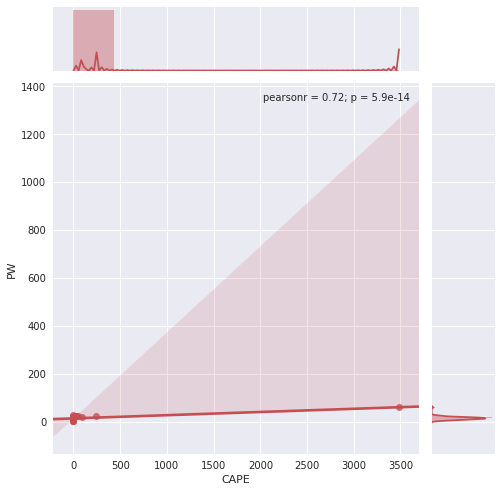
\includegraphics[height=5cm]{Z002.png}
    
    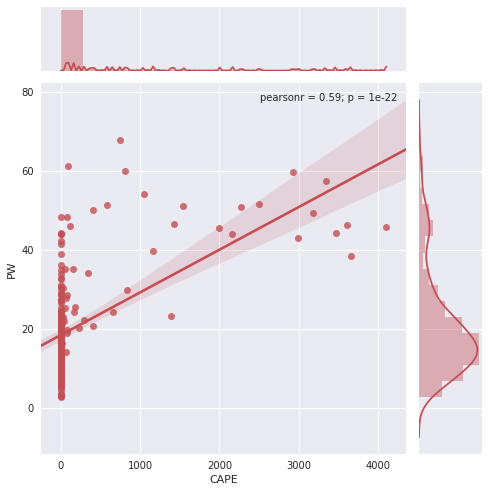
\includegraphics[height=5cm]{Z122.png}
    
    \textit{Gráfica PW contra CAPE}
\end{center}


Vemos que a las 12:00 horas, CAPE se mantiene relativamente reducido, hasta que PW se eleva por encima de los 40 mm.

\begin{center}
	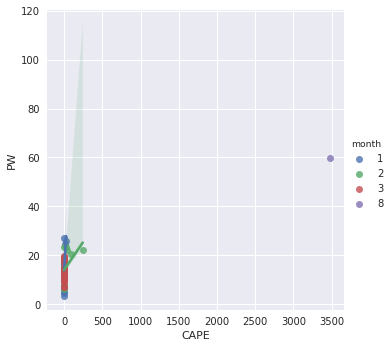
\includegraphics[height=5cm]{Z003.png}
    
    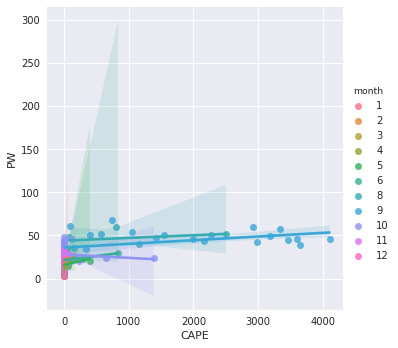
\includegraphics[height=5cm]{Z123.png}

	\textit{Gráfica PW contra CAPE, color distingue cada mes}
\end{center}

Al igual que anteriormente, CAPE se eleva cuando PW supera aproximadamente 40 mm, pero muestra información adicional, mostrando que esto ocurre en los meses de agosto y septiembre.

\section{Conclusiones}

Se enfrentó con la limitación de los datos recibidos, en muchos lugares incompleto, extenso y formatos no compatibles para leer con programas, sin embargo, fue posible obtener información de los datos, realizando una limpieza y adaptación de ellos, y creando gráficas de lo obtenido para analizar claramente la información. Se encontró que CAPE se eleva Empalme, Sonora, a las 12:00 horas, en los meses de agosto y septiembre, Y además que PW se encuentre por encima de 40 mm.

\section{Bibliografía}

\begin{itemize}
\item (2018). Convective available potential energy. 4 de Marzo, 2018, de Wikipedia Sitio web: 

https://en.wikipedia.org/wiki/Convective\_available\_potential\_energy

\item (2016). Precipitable water. 4 de Marzo, 2018, de Wikipedia Sitio web: 

https://en.wikipedia.org/wiki/Precipitable\_water

\item (2016). Fluid parcel. 4 de Marzo, 2018, de Wikipedia Sitio web: 

https://en.wikipedia.org/wiki/Fluid\_parcel
\end{itemize}



\section{Apéndice}

\begin{itemize}
	\item     ¿Cómo se te hizo esta actividad? ¿Compleja, Difícil, Sencilla?

Al inicio no era evidente que acción realizaba exactamente cada paso de la limpieza de datos, pero una vez comprendido y utilizado, se muestra la utilidad que trae.

	\item     ¿Qué te llamó más la atención?
    
La automatización de acciones manuales por emacs
    
	\item     ¿Qué parte fue la que menos te interesó hacer?
    
La actividad fue bastante interesante y útil, ninguna parte específica fue de menos interesante
    
	\item     ¿Cómo mejorarías esta actividad? ¿Qué le faltó? ¿Qué sobró?
    
Brindando una explicación breve en pizarrón, para poder localizar y tomar nota sobre como funcionan los acciones realizadas en emacs que permiten automatizar. No faltó ni sobró información/aprendizaje.
    
	\item     ¿Hasta este punto, que te parece el uso de Jupyter para programar en Python? 
    
Cómodo y rápido, hace buen trabajo en separar acciones por bloques, ejecutarlos y analizar errores en ellos en el momento.
    
    
\end{itemize}




\end{document}